\chapter{Presynaptic Models (Model of neurotransmitter release)}
\label{chap:Presynaptic-models}



This section introduces computational models developed with the goal to
understand the exact mechanism of neurotransmitter release
\begin{itemize}
  \item  whereby Ca2+ enter presynaptic terminal (bouton) through Vm-gated Ca2+
  channels; 
  
  \item the specific proteins with which Ca2+ ions interact, and the detailed
  mechanism leading to exocytosis, i.e. the release of neurotransmitters.
\end{itemize}

The components on presynaptic side is discussed in
Sect.\ref{sec:presynaptic-side-structure} and Sect.\ref{sec:both-side-synapse}.

\section{Neurotransmitter concentrations}
\label{sec:neurotransmitter-concentration}

\subsection{Glutamate}
\label{sec:Glutamate-concentration}

The concentration of glutamate varies dramatically depending upon the biological
compartment being measured:  plasma glutamate levels are estimated in the range
of 150 $\muM$, cerebrospinal fluid levels around 10 $\muM$, and intracellular
glutamate concentrations in the brain are approximately 10 mM (Danbolt, 2001; Featherstone
and Shippy, 2008).  

When doing experiments: more mature neurons will tolerate higher glutamate
concentrations, so time in culture is important. 

\begin{enumerate}
  \item In the synaptic cleft:
  \begin{itemize}
     \item Resting = few micromolar , e.g. 5uM
     
     Reported values of baseline glutamate concentrations range up to 4 $\mum$.
     However, in acute hippocampal slices, Herman and Jahr found that the
     concentration is much lower, near 25 nM (Herman, Jahr, 2007). 
     %http://www.jneurosci.org/content/27/36/9736
     
     NOTE:  If glutamate were present tonically at low micromolar
     concentrations, many receptors, especially the high-affinity NMDA receptors
     (NMDARs), would be activated or desensitized, altering neuronal
     excitability as EC50 of NMDAR for glutamate is about 2$\muM$.
          
     \item {\bf in corticostriatal synapse} (MSN):
     
     
     
     The synaptic cleft is 14nm height; with average volume $0.76 \times 10^{-3}
     \mum^3$; with quantal release of 2000 molecules
     (Sect.\ref{sec:synaptic-vesicles}); the peak concentration is 4.3 mM. Yet
     if we consider the effective volume to which neurotransmitter also have
     rapidly access (e.g. the radius 0.5$\mum$ from the center of cleft
     (Schikorski, Stevens, 1997), Moussawi et al., 2011) to which is much bigger
     $44\times 10^{-3} \mu^3$), then the concentration drops to 75 $\muM$.
     
     %2000/(6.022*10^23)/(0.76*1e-3*1e-15))*1e3
     
%      and diameter is about 25-30
%      nm; giving the volume of (14*30*30) nm$^3$.
%      
     %2000/(6.022*10^23)/(0.76*1e-3*1e-15))*1e3
     
     \item {\bf in hippocampal pyramidal neuron}: glutamate concentration can be
     increased up to 1.1 mM in the synaptic cleft ( Per Andersen - Hippocampus
     book, page 224-225) -   at 1.1 mM cultured hippocampal neurons (Clements et
     al., 1992).
     
     %https://books.google.com/books?id=zg6oyF1DziQC&pg=PA224&lpg=PA224&dq=one+vesicle+has+2000+glutamate+molecule&source=bl&ots=iE8l9RNLrB&sig=XrUtrrJQ1AH3uMxh3bw-cMHEKD0&hl=en&sa=X&ved=0ahUKEwjb7ZOg46_UAhXEz4MKHQs5DlsQ6AEISjAG#v=onepage&q=one%20vesicle%20has%202000%20glutamate%20molecule&f=false
     
     
     \item (Dzubay, Jahr, 1999) {\bf in mossy climbing fiber Purkinje cell}:
     synaptic cleft can increase transiently from <20 nM to 1 mM following action potentials in
     climbing fiber (Dzubay, Jahr 1999)
  
     \item {\bf in rod synapse (rod bipolar cell)}: assuming quantal release
     with 2000 molecules per vesicle, and synaptic cleft volume is 0.21 $\mum^3$, then the peak
     concentration is 16 $\muM$ (Rao-Mirotznik et al., 1998) considering
     the cleft width is about 20-40nm with diameter is about 0.4 to 0.8 um.

     Here they assume and a single vesicle contains between 2000 and 5000
     molecules of glutamate (Rao-Mirotznik et al., 1998).
     
     \item consider quantal release of glutamate vesicle which has average
     diameter of 40nm; an estimated glutamate concentration
     of 60 to 210 mM, i.e. about 20,000 molecules
     
     In motor nerve terminal: each vesicle contains 5,000 to 20,000 ACh
     molecules; and an action potentials produce the release of ACh from 10 to
     200 vesicles. \url{http://neuromuscular.wustl.edu/pathol/snare.htm}
     
  %2000/(6.022*10^23)/(4/3*3.14*40^3*1e-24))*1e3
  % 2000 = #molecule/vesicle
  % convert to mole --> devidied by Avogadro number = 6.023*10^23
  %  convert nm^3 to liter --> 1e-24
  %  result is Molar --> convert to mM by multiplying 1e3
     
     
     \item time course: which is rapidly decreased in the lapse of milliseconds.
           
  Clements et al. (1992) showed that decay occur with time constant 1.2 ms in
  cultured hippocampal synapses. 
  The concentration cannot be greater than 50 $\muM$ for more than 5ms otherwise
  the rise time of the synaptic current would be affected by the presence of
  D-AA; but this is not the case from the experiment (Clements et al., 1992).
  
  \end{itemize}

  \item In the extrasynaptic space: extrasynaptic transmitter concentration
  reaches 160-190 microM.

The estimates of the tonic basal concentration of glutamate within the
extracellular space outside of the synaptic cleft varies over three orders of
magnitude, ranging from 0.02 to 30 $\muM$ (Herman and Jahr, 2007; Chefer et al.,
2009). The variance in estimated extracellular glutamate concentration results
from electrophysiological estimates made in vitro from tissue slices
(0.02-0.1 $\muM$) versus in vivo measurements using microdialysis or voltammetry
(1-30 $\muM$). It is important to discerning the reason behind this
as the concentration of extracellular glutamate will determine its role in
metabolic processes such as cellular redox potential and neurometabolic
coupling between synaptic activity, glial metabolism, and blood flow (Aoyama et
al., 2008; Magistretti, 2009).

It was estimated that glutamate concentration peaks at $<$250 $\mu$M at the
Bergmann glia membranes (Bergles et al., 1997). Using cyclothiazide (CTZ) to
alter the dose-response relationship of glutamate at Bergmann glia AMPA
receptors, Dzubay and Jahr (1999) estimated that in limbing fiber-Purkinje cell
synaptic clefts, the extrasynaptic transmitter concentration reaches 160-190
microM which, even though much smaller than the peak in the cleft, is still high
enough to activate glutamate receptors. These results indicate that the sphere
of influence of synaptically released glutamate can extend beyond the synaptic cleft.
  
  \item within the neurons::
  \begin{itemize}
    \item 1-10mM : about few thousands time higher than extracellular
    \item 100mM: in the nerve terminal and inside synaptic vesicles, the
    concentration of glutamate can be as high as 100 mM. 
  \end{itemize}
  
\end{enumerate}


\subsection{-- time course}
\label{sec:Glutamate-time-course}
 
CLASSICAL VIEW: released neurotransmitter acts locally on postsynaptic receptors
and is cleared from the synaptic cleft within a few milliseconds by diffusion
and by specific reuptake mechanisms. This rapid clearance restricts the spread
of neurotransmitter and, combined with the low affinities of many ionotropic
receptors, ensures that synaptic transmission occurs in a point-to-point
fashion.

CURRENT VIEW: When transmitter release is enhanced, the concentration of
glutamate increases and its clearance is delayed; this allows it to spread away
from the synapse and to activate presynaptic inhibitory metabotropic glutamate
receptors (mGluRs). At normal levels of glutamate release during low-frequency
activity, these presynaptic receptors are not activated.
\begin{enumerate}
  \item In the hippocampal mossy fibre synapses (Scanziani et al., 1997)
  
  The use-dependent activation of presynaptic mGluRs represents a
  negative-feedback mechanism for controlling the strength of synaptic
  transmission - Sect.\ref{sec:mGluR-presynaptic}.
  
  
\end{enumerate}

The concentration of glutamate reached outside of the cleft after synaptic
release is critical in determining the extent of extrasynaptic receptor
activation.



\section{Simple approaches of Neurotransmitter time-course}
\label{sec:neurotransmitter-time-course}

The  release  of transmitter is quite complex. We can model it at a different
detail level using either (review: Clements et al., 1992; Clements 1996)

\begin{itemize}
  \item using a fixed wave-form of presynaptic voltage and transform it to
  neurotransmitter concentration

\begin{itemize}
  \item square-wave process -
  Sect.\ref{sec:neurotransmitter-time-course-square-wave}
  
  \item single exponential functional form -
  Sect.\ref{sec:neurotransmitter-time-course-single-exponential-decay} 
  
\end{itemize}

\end{itemize}

\subsection{Pulse}
\label{sec:neurotransmitter-time-course-square-wave}

Simple square wave to give $NT=NT_\max$ for a short duration $\Delta t$ (after
which [NT] returns to 0), Fig.\ref{fig:NT-square-wave}.

\def\onset{{\text{onset}}}
\begin{equation}
[NT] = \left\{ \begin{array}{cc}
[NT]_\max  & \text{ if  }  t_\onset < t  < t_\onset + \Delta t \\
0 & \text{ otherwise}
\end{array} \right.
\end{equation}

\begin{figure}[hbt]
 \centerline{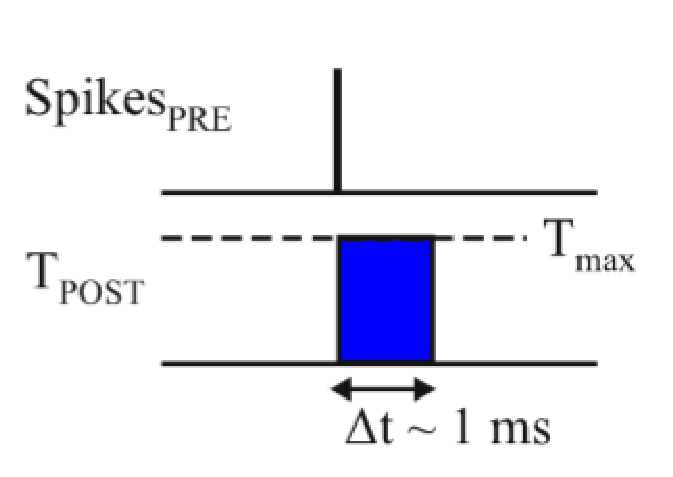
\includegraphics[height=3cm]{./images/NT-square-wave.eps}}
 \caption{Neurotransmitter concentration as a square wave pulse}
\label{fig:NT-square-wave}
\end{figure}


\subsection{Destexhe-Mainen-Sejnowski (1994)}
\label{sec:Destexhe-Mainen-Sejnowski-1994}
\label{sec:neurotransmitter-time-course-single-exponential-decay}

Neurotransmitter concentration [NT] as an instantaneous function of $\Vm$ as
$\Vpre$ to give 

\begin{equation}
[\NT](\Vpre) = \frac{[\NT]_\max}{1 + \exp \left( -(\Vpre - V_p)/K_p \right)}
\end{equation}
with $[\NT]_\max$ = maximal concentration of neurotransmitter -
Sect.\ref{sec:neurotransmitter-concentration}; $\Vpre$ =
presynaptic transmembrane potential; $K_p = 5$ (mV) - the steepness; $V_p =
2$(mV) (voltage at which $[\NT]$ is half-activated). 

% which is modeled as
% \begin{equation}
% [L] = \frac{[L]_\max}{1 + exp( -(\Vm-V_p)/K_p)}
% \end{equation}
% to give $L=L_\max$ for a short duration $\Delta t$ (after which [L] returns to
% 0).

\subsection{Bi-exponential function}

We can model:
\begin{verbatim}
t_rise = 1.22 msec, 
t_decay = 8.34 msec, 

gmax 5 570 pS;
\end{verbatim}


\section{Calcium-induced neurotransmitter release}

A mechanistic representation includes
\begin{verbatim}
channel gating <---> voltage
Ca2+ channel gating <---> [Ca2+]_i

[Ca2+]_i   <----> neurotransmitter release           
\end{verbatim}

\subsection{Yamada-Zucker (1992)}
\label{sec:Yamada-Zucker-1992}

Assumption:
\begin{itemize}
  \item $\Ca$ influx via high-threshold voltage-activated $\Ca$ channel (HVA
  $\Ca$ channel)
  
  \item $[\Ca]$ increase, enable $\Ca$ binding to a special protein, i.e.
  each activated $\Ca$-bound protein then binding to transmitter-containing
  vesicles and promotes release of $n$ neurotransmitter for each vesicle.
  
  \item it requires 4 $\Ca$ ions for activating $\Ca$-binding protein
  
  \item {\bf inexhaustible} supply of neurotransmitter
  
  \item concentration of NT is assumed uniform in the cleft, and is cleared by a
  passive diffusion outside the cleft, with a rate constant $k_c$
\end{itemize}

\begin{equation}
\begin{split}
\ce{4Ca^2+ + X <=>[k_b][k_u] X*} \\
\ce{X* + V_e <=>[k_1][k_2]  V_e^* ->[k_1] n }\NT \\
\NT \ce{->[k_c]} \ldots
\end{split}
\end{equation}
with $X$ represent the amount of $\Ca$-binding protein.

\begin{itemize}
  \item $k_b = 10^5$ (1/(sec.mM$^4$)) = 100 (1/(ms.mM$^4$))
  
  \item $k_u = 100$ (1/sec) = 0.1 (1/(ms.mM$^4$))
  
  \item $k_1 = 10^6$ (1/(sec.mM)) = $10^3$ (1/(ms.mM))
  
  \item $k_2 = 100$ (1/sec) = 0.1 (1/ms)
  
  \item $k_3 = 4,000$ (1/sec) = 4 (1/ms)
  
  \item $V_e = 0.01$ (mM) = concentration of vesicles
  
  \item $k_c = 10^4$ (1/sec) = 10 (1/ms) 
  
  \item $[X]_\max = 0.001$ (mM) = maximal concentration of $\Ca$-binding protein
  
  \item $n=10,000$ : the number of neurotransmitters per vesicle
\end{itemize}